\section{Durchführung}
\label{sec:Durchführung}

Die Durchführung dieses Versuches beinhaltet zwei unteschiedliche Messprozesse. Beide Messprozesse können mit ähnlichen Versuchsaufbauten vollzogen werden. Bei dieser Messung
werden Kennlinien und das Anlaufstromgebiet einer Vakuumdiode aufgenommen. Aufgrund der sehr kleinen Ströme im Anlaufstromgebiet können äußere Bedingungen großen Einfluss
auf die Messung haben, weshalb gute Umweltbedingungen für eine qualitative Messung nötig sind. 

\subsection{Aufnahme der Kennlinien einer Hochvakuumdiode}
\label{subsec:D_Kennlinien}
Die Kennlinien einer Hochvakuumdiode können mit einem Versuchsaufbau nach \autoref{fig:Schaltplan1} aufgenommen werden. Dabei befindet sich in der Hochvakuumdiode ein Glühdraht.
An diesem liegt eine Heizspannung an, sodass durch den glühelektrischen Effekt Elektronenemission stattfinden kann. Weiter liegt zwischen dem Glühdraht und der Anode eine 
Spannung an. Durch diese können die Elektronen zu Anode gelangen und somit einen Strom erzeugen, welcher an dem eingezeichnetem \textit{Amperémeter} gemessen werden kann.
\begin{figure}
    \centering
    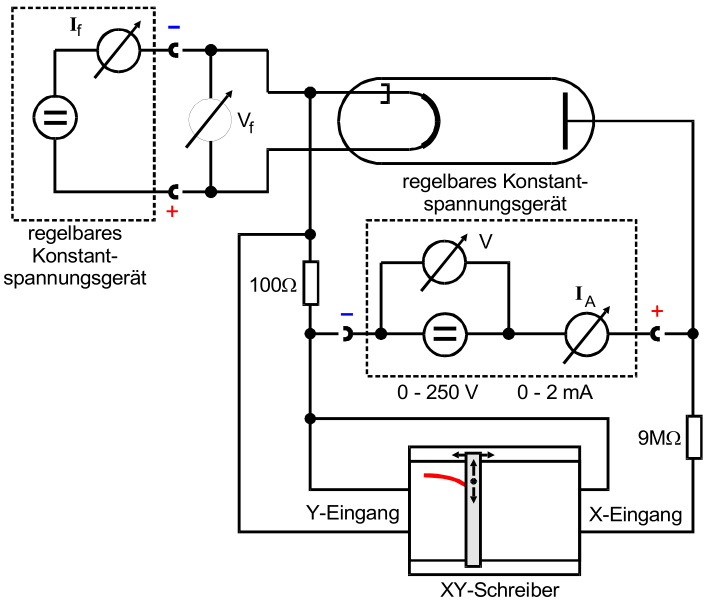
\includegraphics[width = .6\textwidth]{content/Schaltplan1.png}
    \caption{Schaltplan zur Vermessung der Kennlinien der Hochvakuumdiode \cite{v504}.}
    \label{fig:Schaltplan1}
\end{figure}
Um nun die Kennlinie der Hochvakuumdiode aufzunehmen wird ein Heizstrom von $\qty{2}{\ampere}$ bis $\qty{2.5}{\ampere}$ angelegt. Dieses Intevall muss eingehalten werden, da
der Draht Ströme größer als $\qty{2.5}{\ampere}$ nicht aushält. Allerdings haben die Messwerte erst ab circa $\qty{1.9}{\ampere}$ die nötige Qualität. Die Heizspannung wird 
mit einem seperaten \textit{Voltmeter} gemessen. Das \textit{Voltmeter} muss mindestens eine Auflösung von $\qty{0.1}{\volt}$ haben. Nun werden die Heizstromstärke $I_{text{H}}$
und die zugehörige Heizspannung $U_\text{H}$ notiert. Dann wird die Beschleunigungsspannung $U_\text{B}$ erhöht und es werden Wertepaare von $I_\text{H}$ und $U_\text{B}$ 
notiert. Dabei wird ein Spannungsintervall von $[0,250]\unit{\volt}$ durchlaufen. Dabei soll bei größeren Veränderungen der Stromstärke detaillierter gemessen werden. Dieser 
Messprozess wird für fünf verschiedene Heizströme wiederholt. Darunter sollte sich auch der maximale Heizstrom befinden. Kann bei den aufgenommenen Messreihen kein 
Sättigungsstrom erkannt werden muss der Prozess wiederholt werden. 
\subsection{Aufnahme des Anlaufstromgebietes}
\label{subsec:Anlaufstromgebiet}
Das Anlaufstromgebiet kann durch den Versuchsaufbau in \autoref{fig:Schaltplan2} durchgeführt werden. Nun wird für die Beschleunigungsspannung ein Spannungsgenerator verwendet, 
welcher ein Intervall von $\qty{0}{\volt}$ bis $\qty{1}{\volt}$ in $\qty{0.1}{\volt}$-Schritten durchlaufen kann. Da die Ströme im Anlaufstromgebiet sehr klein sind wird ein
sehr hochauflösendes \textit{Amperémeter} verwendet. Bei dieser Messung ist die korrekte Polung am Heizdraht wichtig. Außerdem muss vor Beginn der Messung der 
Übergangswiderstand minimiert werden. 
\begin{figure}
    \centering
    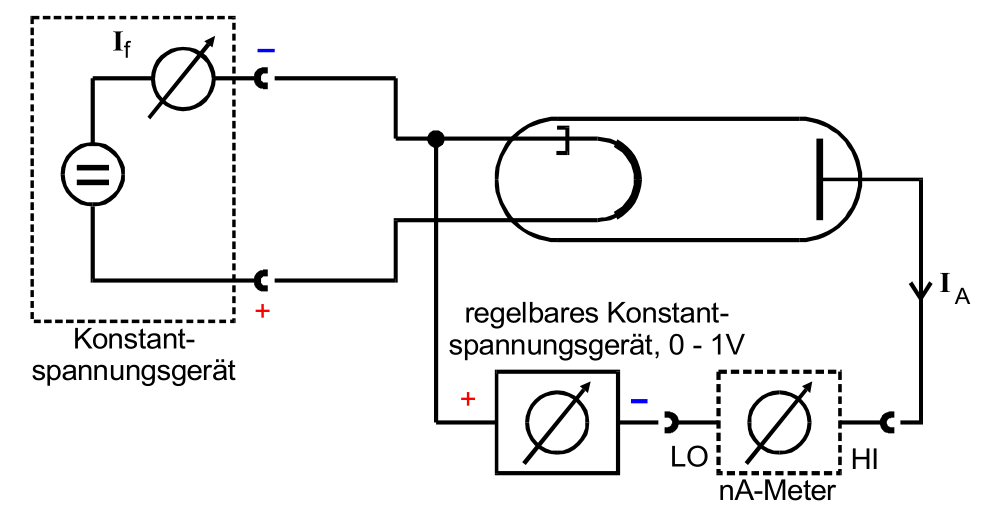
\includegraphics[width = .6\textwidth]{content/Schaltplan2.png}
    \caption{Schaltplan zur Vermessung des Anlaufstromgebietes der Hochvakuumdiode \cite{v504}.}
    \label{fig:Schaltplan2}
\end{figure}
Nun wird das beschriebene Intervall durchlaufen. Dabei werden Anlaufstrom und Beschleunigungsspannung notiert. Für die Auswertung dieses Versuches ist es wichtig den 
Innenwiderstand des Messgerätes zu notieren, da anhand dessen eine Korrektur der Werte vorgenommen werden muss.